\label{chapter2}
\chapter{Definitions}

Author \cite{Review2021} defines terms as following

\begin{itemize}
	\item Residential: private residences, with no commercial usage, occupied by one or more persons either full-time or part-time during a calendar year.
	\item Load: the electricity that all the electricity-powered devices in the household consume in unit time.
	\item Profile: a graph representing the significant features of the electricity load over time.
	\item Model: "a formal system that represents the combined processes" \cite{KAVOUSIAN2013184} of electricity consumption by all the electricity-powered devices in a private residence/number of residences.
\end{itemize}

Commonly load profile is a term defined as aggregated power usage of all appliances in a house. 
Sometimes load profile is used to describe appliance-level load profiles. 
The load profile is most commonly presented with a curve, that shows daily power usage.

\begin{figure}[H]
	\centering
	\caption{"Clustered load profiles. The graph was published by \protect\cite{GERBEC2005}"}
	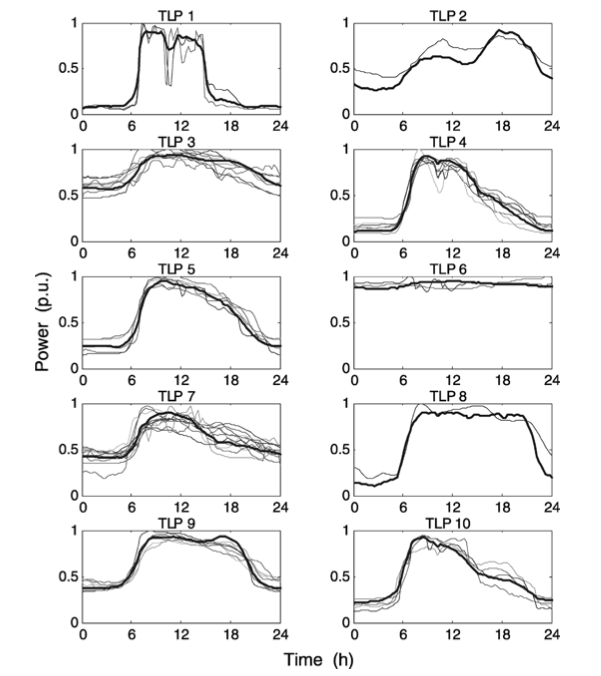
\includegraphics[width=0.9\textwidth]{Figures/clustered_profiles.png}
	\label{fig:profiles}
\end{figure}

Figure \ref{fig:profiles} depicts 10 clusters of daily load profiles. 
This is not the only way to present it, for example, author \cite{Park2019} used an image-based presentation.
In the following chapters we will showcase how we can use various load profiles to present the data. 